\documentclass{atistandalonetask}
\usepackage{atistandard}
\begin{document}
  \begin{atiTask}[
    title = Ionenkristalle
  ]
    \begin{atiSubtasks}
    	\item Skizzieren Sie die Ladungsverteilung 
    	\[
    	\rho(x,y,z)=q\delta(x)\delta(y)[2\delta(z)-3\delta(z+3)]
    	\]
    	und schreiben Sie diese in Zylinderkoordinaten um. 
    	\item Geben Sie die Flächenladungsdichte $\eta(x,y)$ und die Raumladungsdichte $\rho(x,y,z)$ des in der Abbildung gegebenen zweimdimensionalen Kristalls an.
    	\begin{figure}
		\centering
		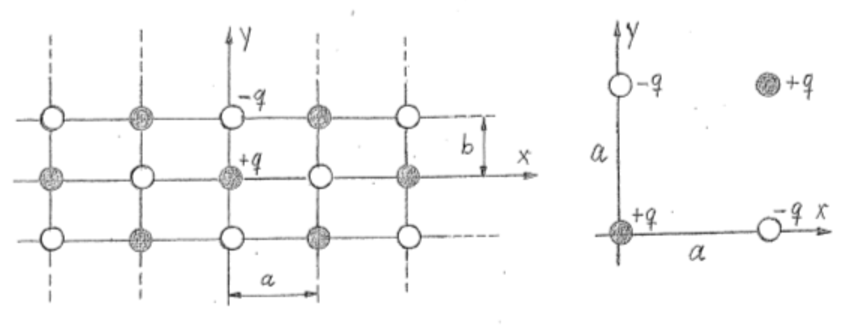
\includegraphics[width=0.7\linewidth]{./picture-delta_v}
		\caption{Links: zu Aufgabe (b), rechts: zu Aufgabe (c)}
		\end{figure}
    	\item Berechnen Sie das elektrische Monopolmoment
    	\[
    %	\int_{-\infty}^\infty\int_{-\infty}^\infty\int_{-\infty}^\infty
    	\iiint\limits_V\rho(x,y,z)\D V
    	\]
    	und das Dipolmoment
    	\[
    	%\int_{-\infty}^\infty\int_{-\infty}^\infty\int_{-\infty}^\infty
    	\iiint\limits_V\vec{r}\rho(x,y,z)\D V
    	\]
    	über den gesamten Raum.
    \end{atiSubtasks}	
  \end{atiTask}
  \begin{atiSolution}
   	Lösung folgt
  	%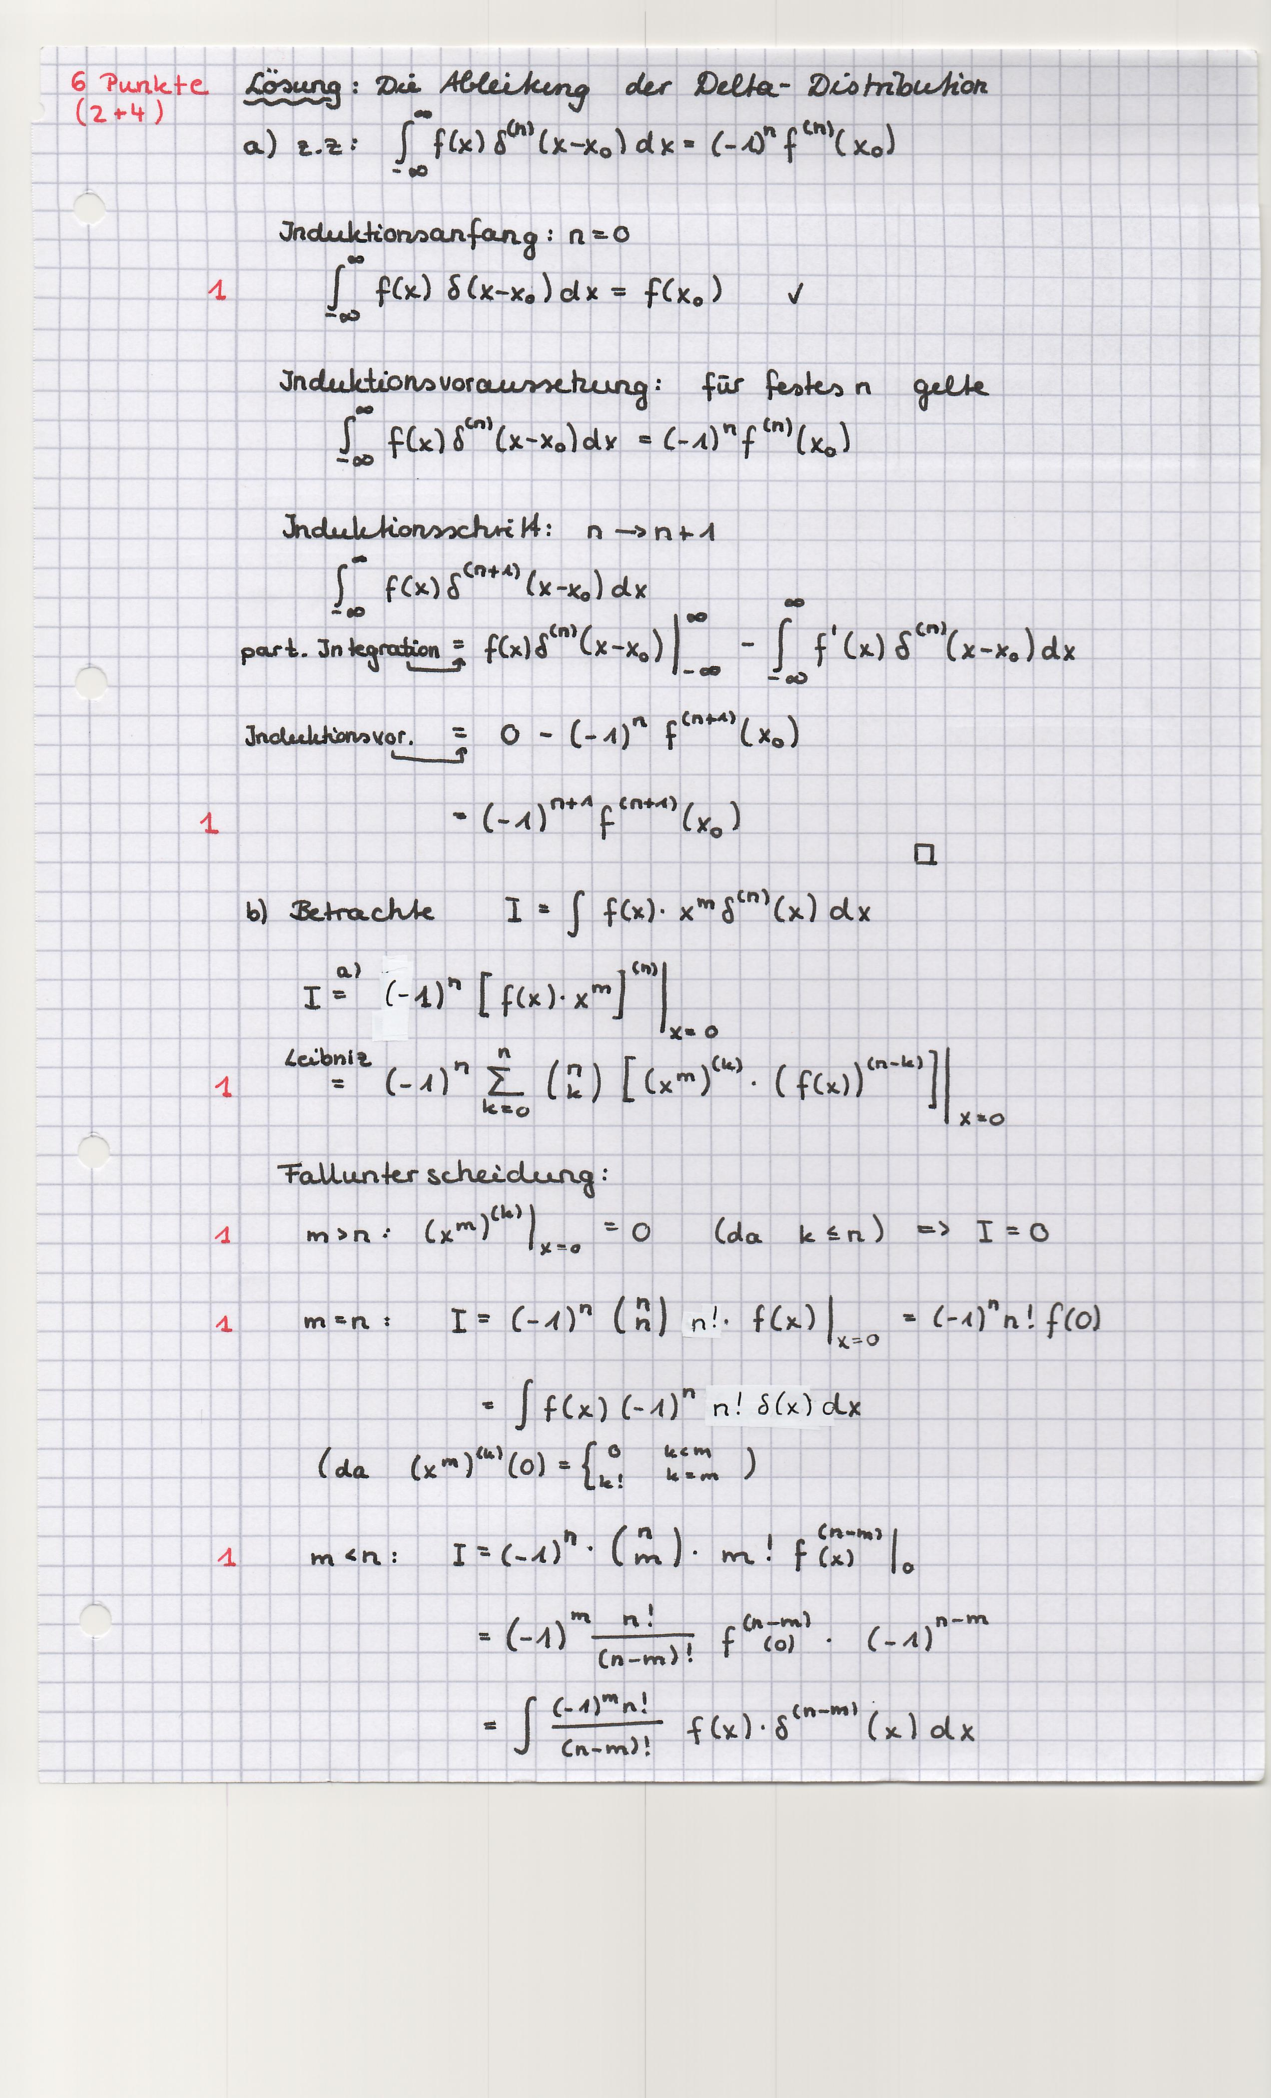
\includepdf[pages=-]{solution-delta_iv.pdf}
  \end{atiSolution}
\end{document}